\section{System Modeling and Actuators}

\setcounter{section}{3}
\setcounter{subsection}{1}
\subsection{Electrical Motors} %% -------------------------- 3 . 2 -------------

\textbf{Basic equations}. Let \(\omega_m\) be the angular velocity of the motor
shaft, \(T\) the motor torque, \(T_L\) the torque of the load, \(J_m\) the
rotational inertia in the motor, \(P_m\) the power delivered from the motor the
shaft and \(P_L\) the mechanical power delivered to the load, then
\begin{align*}
    J_m\dot{\omega}_m &= T - T_L \\
    P_m & = T\omega_m \\
    P_L & = T_L\omega_m
\end{align*}

\textbf{Gears}
\begin{align*}
    \omega_{out} &= n\omega_{in} \\
    T_{out} &= \frac{1}{n}T_{in} \\
    P_{in} = T_{in}\omega_{in} &= T_{out}\omega_{out} = P_{out}
\end{align*}

\textbf{Motor and gear}
\begin{Figure}
    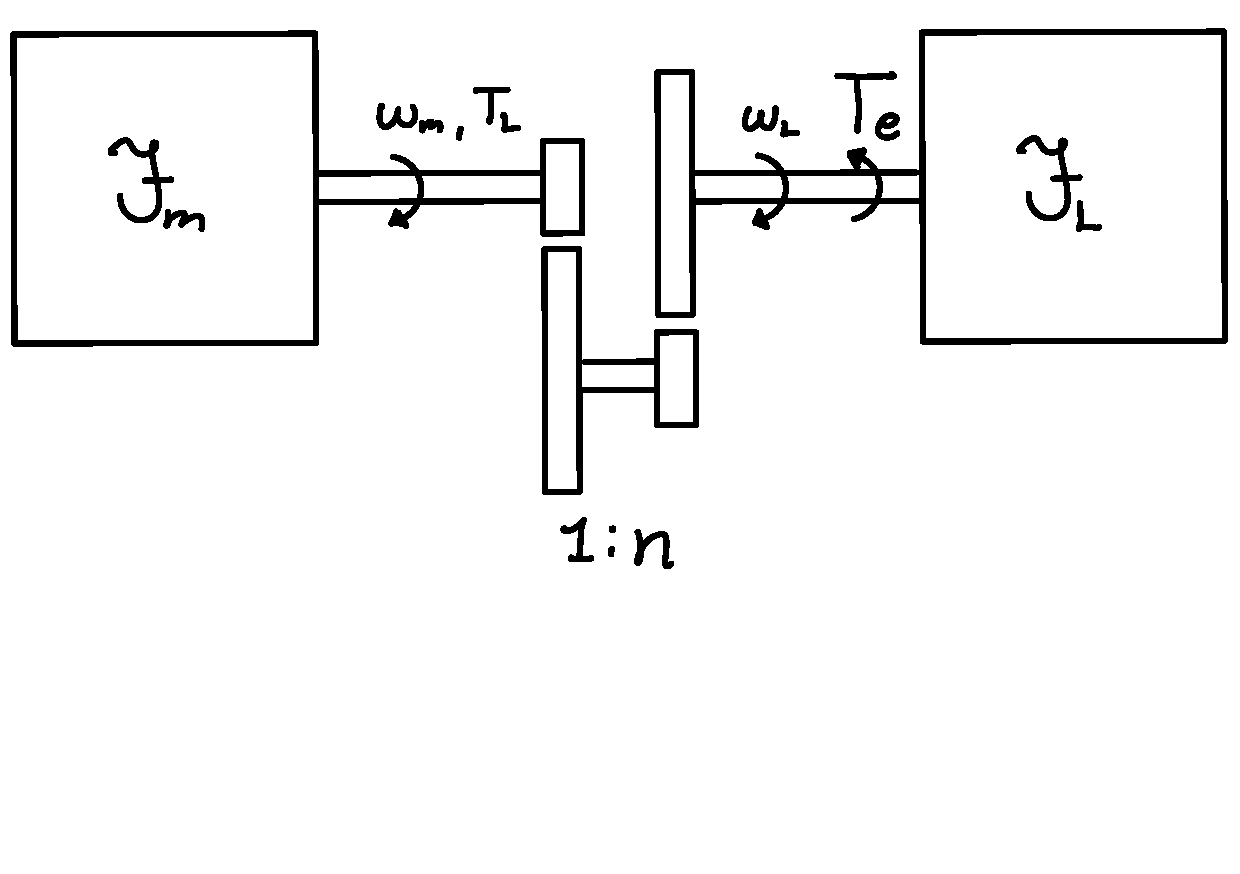
\includegraphics[clip, trim = 0cm 5cm 0cm 0cm,width=\linewidth]{figures/gears.pdf}
    \label{fig:gears}
\end{Figure}
\begin{align*}
    (J_m+n^2J_L)\dot{\omega}_m = T - nT_e
\end{align*}

\textbf{Torque characteristics}
The motor torque \(T\) and the torque of the load \(T_L\) are often functions of
the motor speed \(\omega_m\).
\begin{align*}
    &T_L(\omega_m) &  &T(\omega_m)
\end{align*}
Stability can be investigated in a torque-speed diagram
\begin{align*}
    k = \left(\frac{\partial T}{\partial \omega_m} - \frac{\partial T_L}{\partial \omega_m}\right)\Big|_{\omega_m}
\end{align*}
The system is stable in an equilibrium point \(T_L(\omega_m) = T(\omega_m)\) if \(k\leq 0\)
\newline

\textbf{The four quadrants of the motor}
A motor can both deliver and receive power, it can act as both a motor and a 
generator.
\begin{align*}
    P = T\omega
\end{align*}

\subsection{The DC motor with constant field} %% ----------- 3 . 3 -------------
\begin{Figure}
    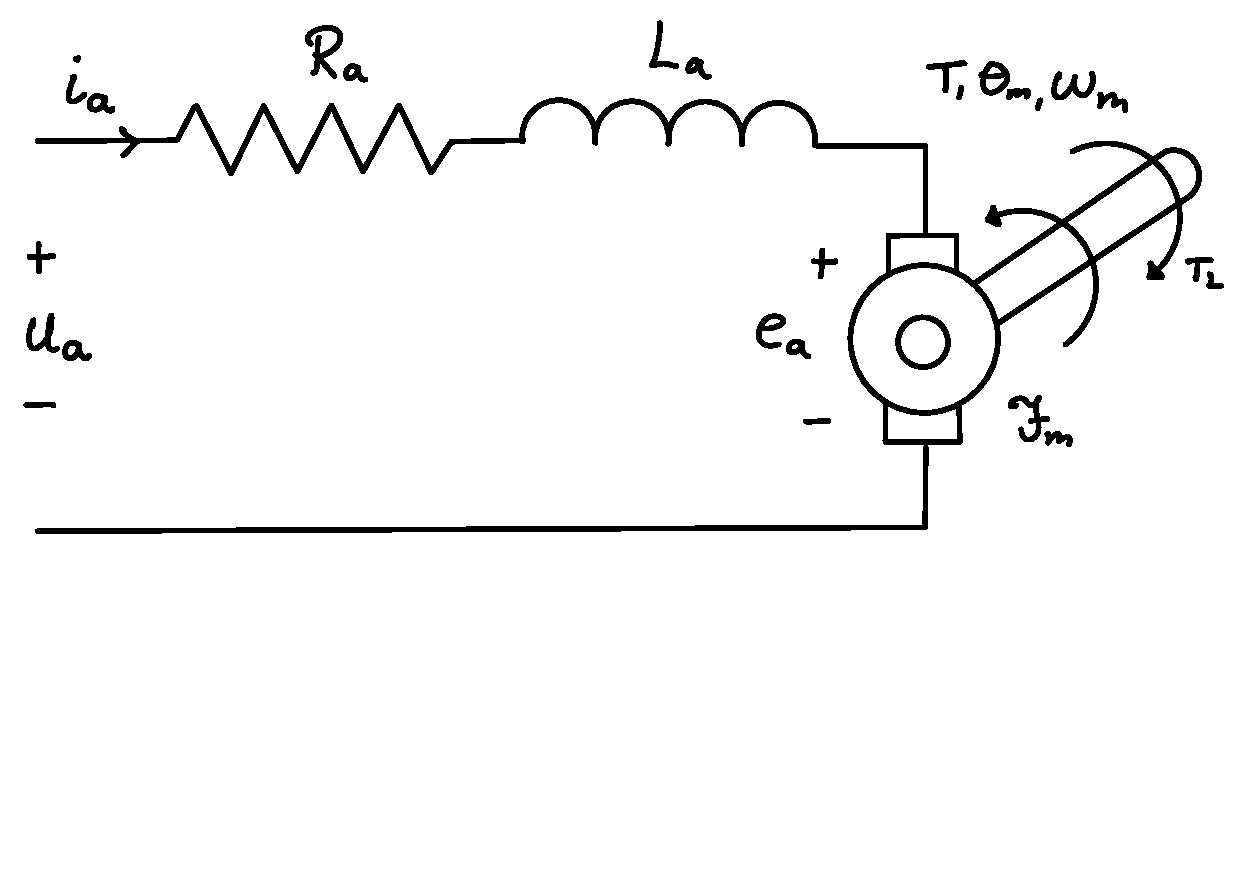
\includegraphics[clip, trim = 0cm 5cm 0cm 0cm,width=\linewidth]{figures/dc-motor.pdf}
    \label{fig:dc-motor}
\end{Figure}
\begin{align*}
    L_a\frac{d}{dt}i_a &= -R_a i_a - K_E \omega_m + u_a \\
    J_m \dot{\omega}_m &= K_T i_a - T_L \\
    \dot{\theta}_m &= \omega_m
\end{align*}
\(K_T\) and \(K_E\) defined by
\begin{align*}
    T&=K_T i_a  & K_E &=  K_T
\end{align*}

\setcounter{subsection}{4}
\subsection{Motor and load with elastic transmission} %% --- 3 . 5 -------------
\begin{Figure}
    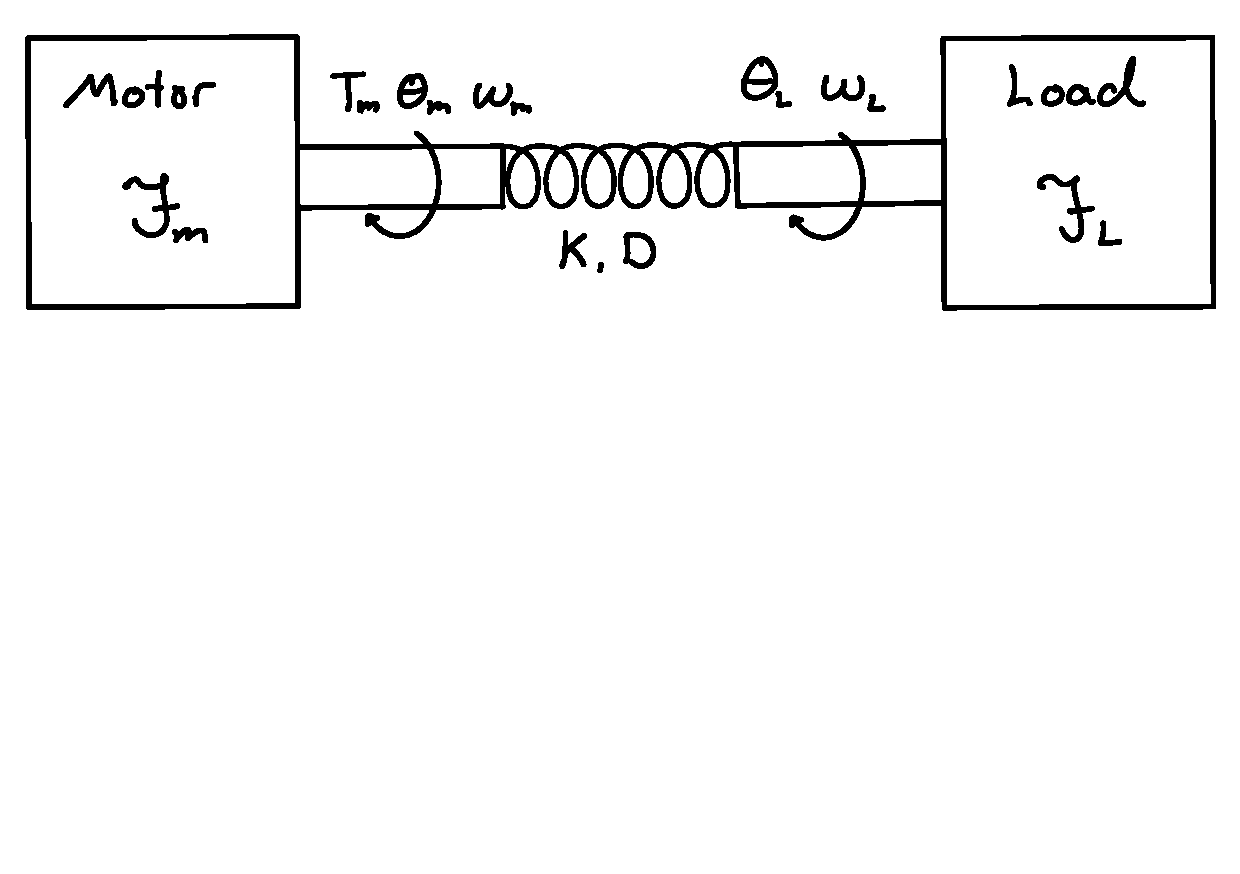
\includegraphics[clip, trim = 0cm 9cm 0cm 0cm,width=\linewidth]{figures/motor-load.pdf}
    \label{fig:motor-load}
\end{Figure}
Spring is damped
\begin{align*}
    \theta_e &= \theta_L - \theta_m & T_L &= -K\theta_e - D\dot{\theta}_e
\end{align*}
The equations are
\begin{align*}
    \ddot{\theta}_e + \frac{D}{J_e}\dot{\theta}_e + \frac{K}{J_e}\theta_e &= -\frac{1}{J_m} T_m \\
    \ddot{\theta}_r &= \frac{T_m}{J_m}
\end{align*}
where
\begin{align*}
    J_e &= \frac{J_m J_L}{J_m + J_L} & \theta_r &= \theta_m + \frac{J_L}{J_m}\theta_L
\end{align*}

\setcounter{section}{4}
\setcounter{subsection}{1}
\subsection{Valves} %% ------------------------------------- 4 . 2 -------------

\textbf{Pressure conversion rules}
\begin{itemize}
    \item \(1\) Pa \(= 1\) N/m\(^2\)
    \item \(1\) bar \(= 10^5\) Pa
    \item \(1\) atm \(= 1.01325\cdot10^5\) Pa
    \item \(1\) psi \(= 6897\) Pa
\end{itemize}

\textbf{Flow through restriction}
The flow \(q\) [kg/m\(^3\)] is related to the density of the fluid \(\rho\), the
change in pressure \(\Delta p\), the cross sectional area of the orifice \(A\)
and the discharge coefficient \(C_d\)
\begin{align*}
    q \approx C_d A \sqrt{\frac{2}{\rho}\Delta p}
\end{align*}
\(C_d = 1\) when no energy is lost, in practice \(C_d \in [0.60, 0.65]\) for orifices
with sharpe edges and \(C_d \in [0.8,0.9]\) with rounded edges.
\newline

\textbf{Reynolds number for flow through restrictions}
\begin{align*}
    R_e = \frac{D}{A\nu}q
\end{align*}
\(D\) is diameter of the restriction, \(A\) is the cross sectional area of the flow,
\(\nu\) is the kinematic viscosity and is approximately \(30\cdot10^{-6}\) m\(^2\)/s
for hydraulic oil. When \(R_e > 1000\) the flow will be turbulent and the formula
for the flow \(q\) is as stated above. When \(R_e < 10\) the flow will be laminar
and
\begin{align*}
    q=C_l \Delta p
\end{align*}

\subsection{Motor models} %% ------------------------------- 4 . 3 -------------

\setcounter{section}{7}
\setcounter{subsection}{0}
\subsection{system modeling}

\textbf{Generalization of concepts across fields}
\begin{itemize}
    \item \(e\) - \textbf{Effort}
    \item \(f\) - \textbf{Flow}
    \item \(I\) - \textbf{Inertance}. 
    \item \(P\) - \textbf{Power}. \(P=e\cdot f\)
    \item \(p\) - \textbf{Momentum}. \(p = I \cdot f\)
    \item \(q\) - \textbf{Displacement}. \(q = \int f_1 - f_2\)
\end{itemize}
\end{multicols}

\begin{tabular}[h]{ |l|c|c|c|c|c|  }
 \hline
  & Effort & Flow & Inertance & Momentum & Displacement \\ \hline
    Linear Mechanics & $F$ & $v$ & $m$ & $p$ & $x$ \\ \hline
    Angular Mechanics & $T$ & $\omega$ & $J$ & $h$ & $\theta$ \\ \hline
    Hydraulics & $p$ & $q$ & & $\Gamma$ & $V$ \\ \hline
    Electrical & $U$ & $i$ & $L$ & $\lambda$ & $Q$ \\ \hline
\end{tabular}
\newpage

\begin{multicols}{2}
